\documentclass[12pt, a4paper]{article}
\usepackage[top=2cm, bottom=3cm, left=2cm, right=2cm]{geometry}

\usepackage[utf8]{inputenc}
\usepackage{graphicx,wrapfig,amsmath,pdfpages,verbatim}
\usepackage{enumitem}
\usepackage{tabularx, arydshln}
\usepackage{float, subcaption}
\usepackage{multirow, multicol}
\usepackage{fancyhdr}
\usepackage{zref-totpages}
\usepackage{minted}
\usepackage{tcolorbox}
\usepackage{framed}
\usepackage{xcolor}
\usepackage{xassoccnt}
\usepackage{pdfpages}
\usepackage{hyperref}
\usepackage{datetime,calc,tokcycle}
\Characterdirective{\addcytoks{#1\ }}

\newcommand{\customtoday}{
  {\the\year.\twodigit{\the\month}.\twodigit{\the\day}}
  \the\cytoks\unskip}

\newcounter{realpage}
\DeclareAssociatedCounters{page}{realpage}
\AtBeginDocument{%
  \stepcounter{realpage}
}

% Minted settings.
\setminted{fontsize=\footnotesize, baselinestretch=1.5}
\usemintedstyle{borland}

% \newcommand{}[]{}
\renewcommand\tabularxcolumn[1]{m{#1}}
\newcolumntype{Y}{>{\centering\arraybackslash}X}
\newcolumntype{A}{>{\hsize=0.2\textwidth}Y}
\newcolumntype{B}{>{\hsize=0.3\textwidth}Y}

\pagestyle{fancy}
\pagenumbering{gobble}
\fancyhead{}
\fancyhead[L]{\fontsize{8}{12} \selectfont GUIA DE LABORATORIO 06}
\fancyhead[C]{\fontsize{8}{12} \selectfont INGENIERÍA DE CONTROL I}
\fancyhead[R]{\fontsize{8}{12} \selectfont PAG \therealpage/\ztotpages}
\fancypagestyle{titulo}
{
    \fancyhead{}
    \fancyhead[C]{\begin{table}[H]
\begin{tabularx}{\textwidth}{@{}|YYYY|@{}}
\hline
\multicolumn{1}{|c|}{\multirow{3}{*}{
\includegraphics[width=1cm]{Escudo.png}}} & \multicolumn{3}{c|}{UNIVERSIDAD CATÓLICA DE SANTA MARÍA}\\
\multicolumn{1}{|c|}{} & \multicolumn{3}{c|}{ESCUELA PROFESIONAL DE INGENIERÍA ELECTRÓNICA} \\
\cline{2-4} 
\multicolumn{1}{|c|}{} & \multicolumn{1}{c|}{ASIGNATURA} & \multicolumn{1}{c|}{CIRCUITOS ELECTRÓNICOS III} & GUÍA DE LABORATORIO N° 03b\\
\hline  
\multicolumn{3}{|c|}{SEGUNDA FASE:} & Docente (s):\\ 
\multicolumn{3}{|c|}{\multirow{2}{*}{EL PLL COMO BASE DEL SINTETIZADOR}} & Ing. Ronald P. Coaguila Gómez\\
\cline{4-4} 
\multicolumn{3}{|c|}{} & Fecha: \customtoday \\
\hline
\end{tabularx}
\end{table}}
    \newgeometry{bottom=4cm, left=2cm, right=2cm}
    \setlength{\headheight}{129.853pt}
    \renewcommand{\headrulewidth}{0pt}
}

\allowdisplaybreaks

\renewcommand{\theenumi}{\alph{enumi}}

\begin{document}

\thispagestyle{titulo}
\begin{center}
{\large EXPERIENCIA N$^o$1 MULTIVIBRADORES Y CIRCUITOS RESONANTES}
\end{center}

{\Large \href{https://drive.google.com/drive/folders/1fvojh8YbbdQwtmJNgBLz1jIMM7Ws86qz?usp=sharing}{VIDEO EXPLICATIVO}}

\section{OBJETIVO}
Analizar el PLL como base del Sintetizador de Frecuencia.

\section{MARCO TEÓRICO}
\subsection{SÍNTESIS DE FRECUENCIA}
Se puede construir un sintetizador de frecuencia alrededor de un PLL, tal como se muestra en la figura 1. Un divisor de frecuencia se inserta en la salida del VCO y el comparador de fase, para que la señal del lazo al comparador este a la frecuencia fo mientras que la salida es la fase del VCO es Nfo. Esta salida es un múltiplo de la frecuencia de entrada, pero siempre y cuando el lazo este en seguimiento. La señal de entrada puede salir de un oscilador a una f1, con la salida del VCO resultante en Nf1, si el lazo se ajusta para seguimiento a la frecuencia fundamental.

\begin{figure}[H]
    \centering
    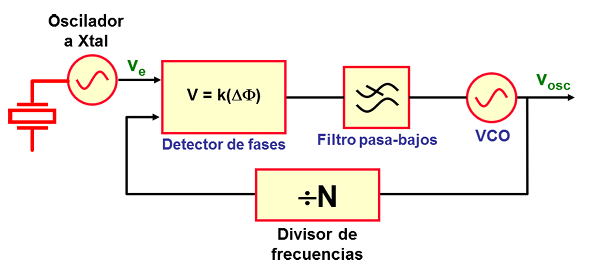
\includegraphics[width=.6\textwidth]{imgs/2.1. Esquemático de un sintetizador.png}
    \caption{Esquemático de un sintetizador}
\end{figure}

En esta experiencia se va a usar un PLL 565 como multiplicador de frecuencia y un 7490 como divisor. La entrada Vi a la frecuencia fo se compara con la entrada en el terminal 5. Una salida a Nfo que ahora es 10fo, se conecta para proporcionar la entrada en la terminal 14 al 7490, la cual varía ente -5 y +5 voltios. Con la salida en el terminal 9, que es la entrada al 7490 dividida entre 10, la señal del terminal del PLL es diez veces la frecuencia de entrada siempre y cuando el lazo permanezca en seguimiento. Debido a que el VCO puede variar solamente a lo largo de un rango limitado respecto a la frecuencia central, puede que sea necesario cambiar la frecuencia del VCO una vez que se cambie el valor del divisor.
\newpage

\section{INFORME PREVIO}

\begin{enumerate}[label=\alph*)]
    \item Analizar y Diseñar un oscilador con un NE555 de 10KHz.\\
    En el modo astable, el temporizador 555 forma una salida continua de señal rectangular con una frecuencia específica que tiene posiciones fijas de la señal de salida en un estado alto y bajo con dos resistencias y un capacitor. Cuando el temporizador 555 en el modo astable recibe energía por primera vez, el capacitor comienza a cargar con voltaje, lo que lleva a una señal de salida alta. Mientras el capacitor se carga hasta llegar a 2/3 del voltaje de suministro del IC. En ese punto, el capacitor comienza a descargarse, lo que lleva a una señal de salida baja. Cuando el voltaje en el capacitor desciende a 1/3 del voltaje de suministro del IC, comienza a cargar nuevamente, lo que lleva a una señal de salida alta y el proceso se repite.\cite{NE555}
    \begin{figure}[H]
        \centering
        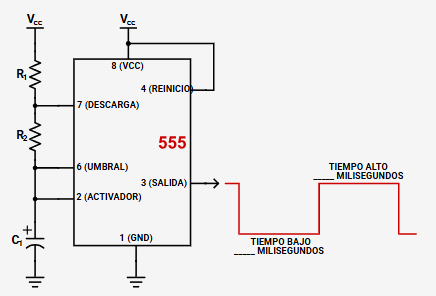
\includegraphics[width=.7\textwidth]{imgs/3.1. 555 Esquemático.png}
        \caption{Esquemático de un oscilado 555 astable}
    \end{figure}
    El comportamiento de un oscilador astable NE555 se describe con las siguientes fórmulas
    \begin{align*}
        T_h&=0.693(R_1+R_2)C_1\\
        T_l&=0.693R_2C_1\\
        f&=\frac{1.44}{(R_1+2R_2)C_1}
    \end{align*}
    Para tener un ciclo de trabajo del 50\%, se selecciona un $R_2$ bastante grande para que $R_1$ haga mucha diferencia entre los tiempos alto y bajos. Para eso, $R_2$ lo seleccionamos como $1M\Omega$. Para que $T_L$ sea cercano $50\mu s$ (para una frecuencia de $10kHz$), se selecciona un capacitor comercial de $68pF$. En consecuencia, $R_1$ podría tomar valores comerciales menores a $5k\Omega$ para mantener una relación cercana al 50\%. Por ejemplo, con $R_1=4.7k\Omega$.
    \begin{align*}
        f = \frac{1.44}{(4.7k+2M)6.8p} = 10.56kHz.
    \end{align*}
    \newpage
    \item Explicar brevemente los tipos de filtros que se usan en un PLL, señalando las ventajas y desventajas de su uso.\\
    Los filtros que acompañan el detector de fase de un PLL son todos pasabajos. Su función es ajustar la respuesta del PLL, haciéndola más rápida o más estable. Cuando el detector de fase es ideal, el filtro no es necesario.
    
    Cuando el comparador de fase no es ideal el filtro pasa a ser necesario. El caso más simple es cuando se trata de un sencillo pasabajos RC, cuya FT es\cite{PLL}:
    \begin{figure}[H]
        \centering
        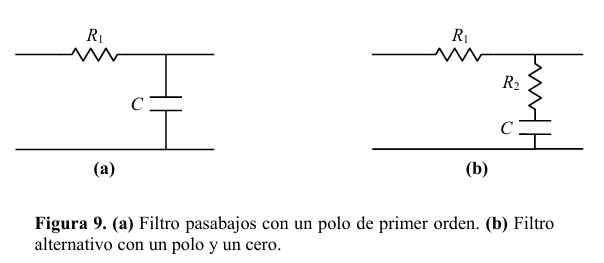
\includegraphics[width=.7\textwidth]{imgs/3.2. PLL Filtros.png}
        \caption{Filtros pasabajos de primer orden\cite{PLL}}
    \end{figure}
    \begin{align*}
        F_1(s)=\frac{1}{1+RCs}
    \end{align*}
    Lo que al introducirse en la función de transferencia del PLL, genera:
    \begin{align*}
        \frac{V_0(s)}{\Omega_i(s)} = \frac{1}{K_{OSC}}\frac{1}{1 + \frac{1}{K_{OSC}K_DA}s + \frac{RC}{K_{OSC}K_DA}s^2}
    \end{align*}
    Lo que da una función de transferencia de segundo orden, con valores característicos:
    \begin{align*}
        \omega_n &= \sqrt{\omega_{RC}K_{OSC}K_DA}\\
        \xi &= \frac{1}{2}\sqrt{\frac{\omega_{RC}}{K_{OSC}K_DA}}
    \end{align*}
    Debe tenerse en cuenta que $\omega_{RC}$ debe ser relativamente pequeño, para poder filtrar la frecuencia $\omega_i + \omega_{VCO} \cong 2\omega_i$. Al mismo tiempo, como $\omega_n$ determina el ancho de banda resultante para el PLL, debe adoptarse lo suficientemente grande para permitir el paso de la máxima frecuencia de variación de la frecuencia de entrada. Esto en general impone limitaciones que se traducen en  bajos valores de $\xi$. La consecuencia será un sistema con una respuesta muy subamortiguada, lo cual no es deseable.

    En caso se tenga un filtro con un polo y un cero, la función de transferencia del filtro sería:
    \begin{align*}
        F_2(s)=\frac{1+R_2Cs}{1+(R_1+R_2)Cs}
    \end{align*}
    Cuyos valores característicos serían:
    \begin{align*}
        \omega_{PLL} \cong \omega_n &= \sqrt{\omega_1K_{OSC}K_DA}\\
        \xi &= \frac{1}{2} \omega_n \left( \frac{\omega_{RC}}{K_{OSC}K_DA} + \frac{1}{\omega_2}\right)
    \end{align*}
    \begin{figure}[H]
        \centering
        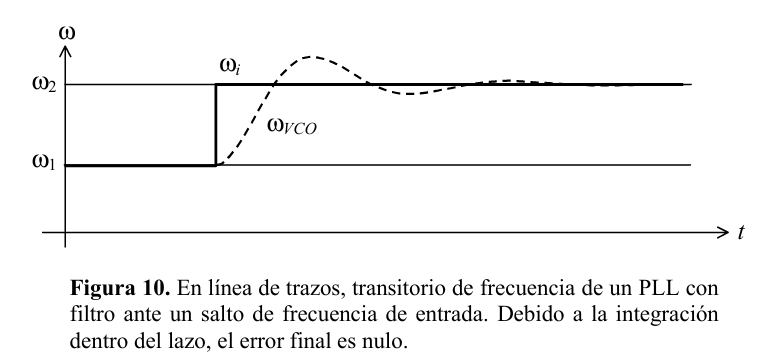
\includegraphics[width=.7\textwidth]{imgs/3.2. Respuesta a un escalón.png}
        \caption{Transitorio de un PLL con un filtro de segundo orden}
    \end{figure}    
    \item Diseñar el filtro más conveniente para este caso.
    \begin{figure}[H]
        \centering
        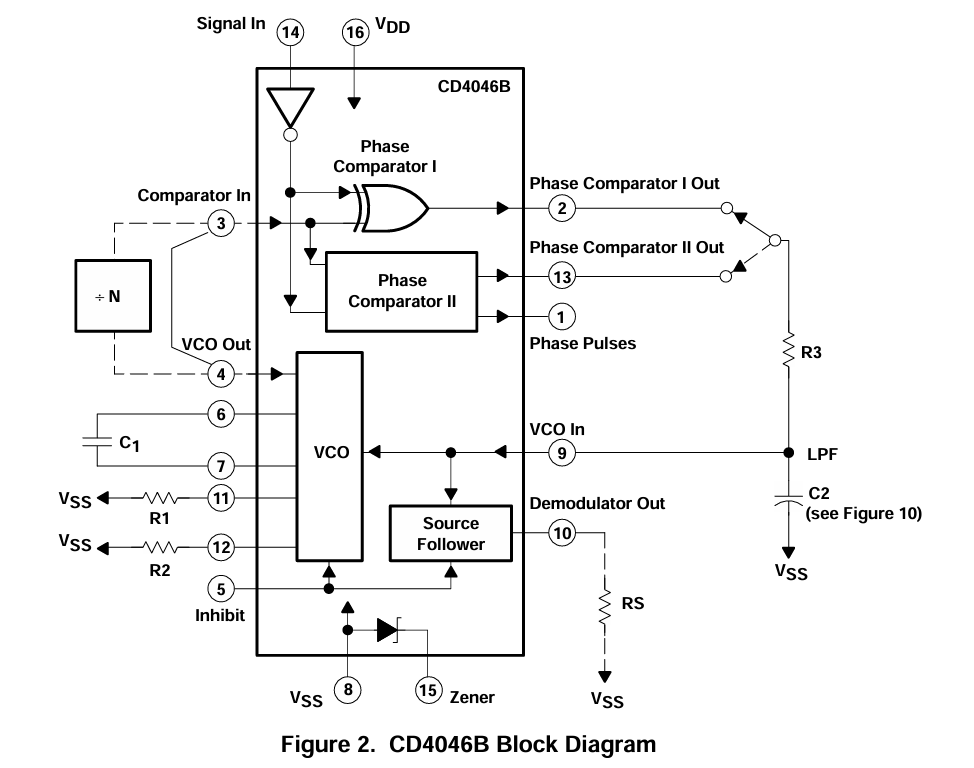
\includegraphics[width=.6\textwidth]{imgs/3.3. Diagrama de bloques del 4046.png}
        \caption{Diagrama de bloques del 4046}
    \end{figure}
    Para el filtro pasabajos (LPF) entre los pines 2/13 y 9, se tomó en cuenta el que PLL 4046 fue diseñado para tener un rango de captura de (según datasheet):
    \begin{align}
        f_c \approx \pm \left( \frac{1}{2\pi} \right) \left( \frac{2\pi f1}{R_3C_2} \right) = \pm 0.4kHz
    \end{align}
    Para la aplicación se eligió un filtro con cero y un polo, de forma que $R_3$ es $27k\Omega$, y en la rama de $C_2$, se coloca un resistor en serie de $330\Omega$ y se elige un $C_2$ de $4.7\mu\Omega$
    \item Explicar brevemente la función de los divisores de frecuencia y las posibilidades de división de un 7493 y un PIC16f628A.
    \begin{figure}[H]
        \centering
        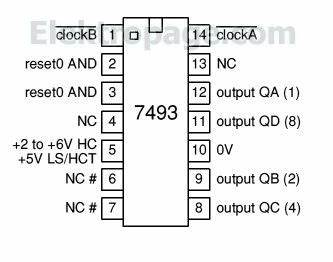
\includegraphics[width=.5\textwidth]{imgs/3.4. 7493 pinout.jpg}
        \caption{7493 pinout}
    \end{figure}
    Teniendo como entrada clockA, y conectando la entrada clockB a la salida output QA, se puede tener 4 salidas:
    \begin{itemize}
        \item Divisor por 1: QA (pin 12)
        \item Divisor por 2: QB (pin 9)
        \item Divisor por 4: QC (pin 8)
        \item Divisor por 8: QD (pin 11)
    \end{itemize}
    \begin{figure}[H]
        \centering
        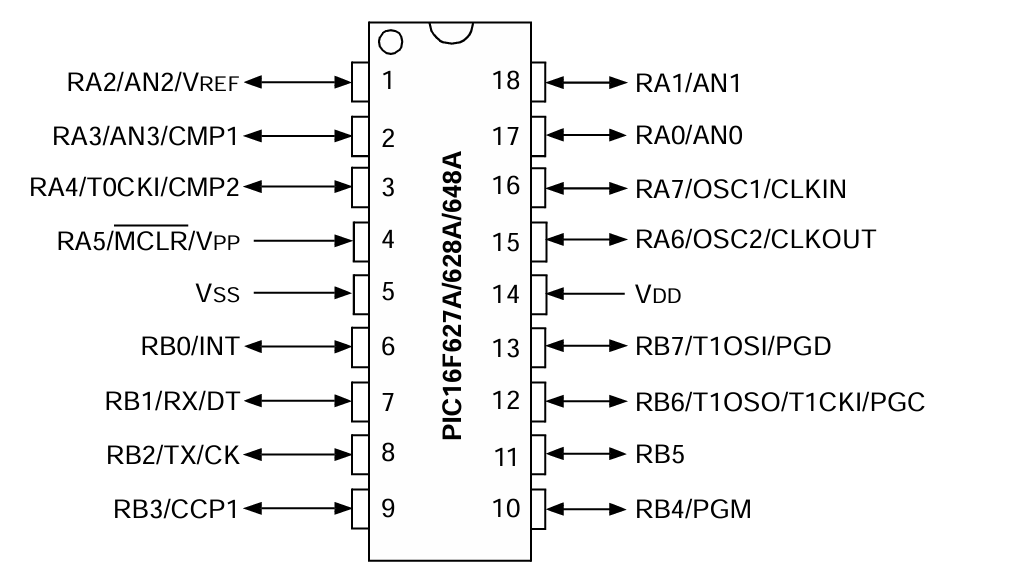
\includegraphics[width=.5\textwidth]{imgs/3.4. 16F628A pinout.png}
        \caption{16F628A pinout}
    \end{figure}
    De los 16 pines I/O digitales, repartidos en los registros A y B, del PIC16f628A, un acercamiento sencillo para la división de frecuencia sería contar la cantidad de flancos en un pin de entrada y después de un número determinado de ellos se genere un flanco, o cambio de estado, en otro pin de salida. Para permitir una división de frecuencia ajustable por el usuario, se pude cnfigurar que los pines de entrada/salida del divisor se encuentren en un solo registro  (por ejemplo, el A) y el otro registro por completo sea utilizado para determinar la cantidad de flancos que se deben contar antes de cambiar el estado del pin de salida, a modo de referencia.
    \item Utilizar un simulador para observar el comportamiento de los circuitos diseñados y propuestos
    \begin{figure}[H]
        \centering
        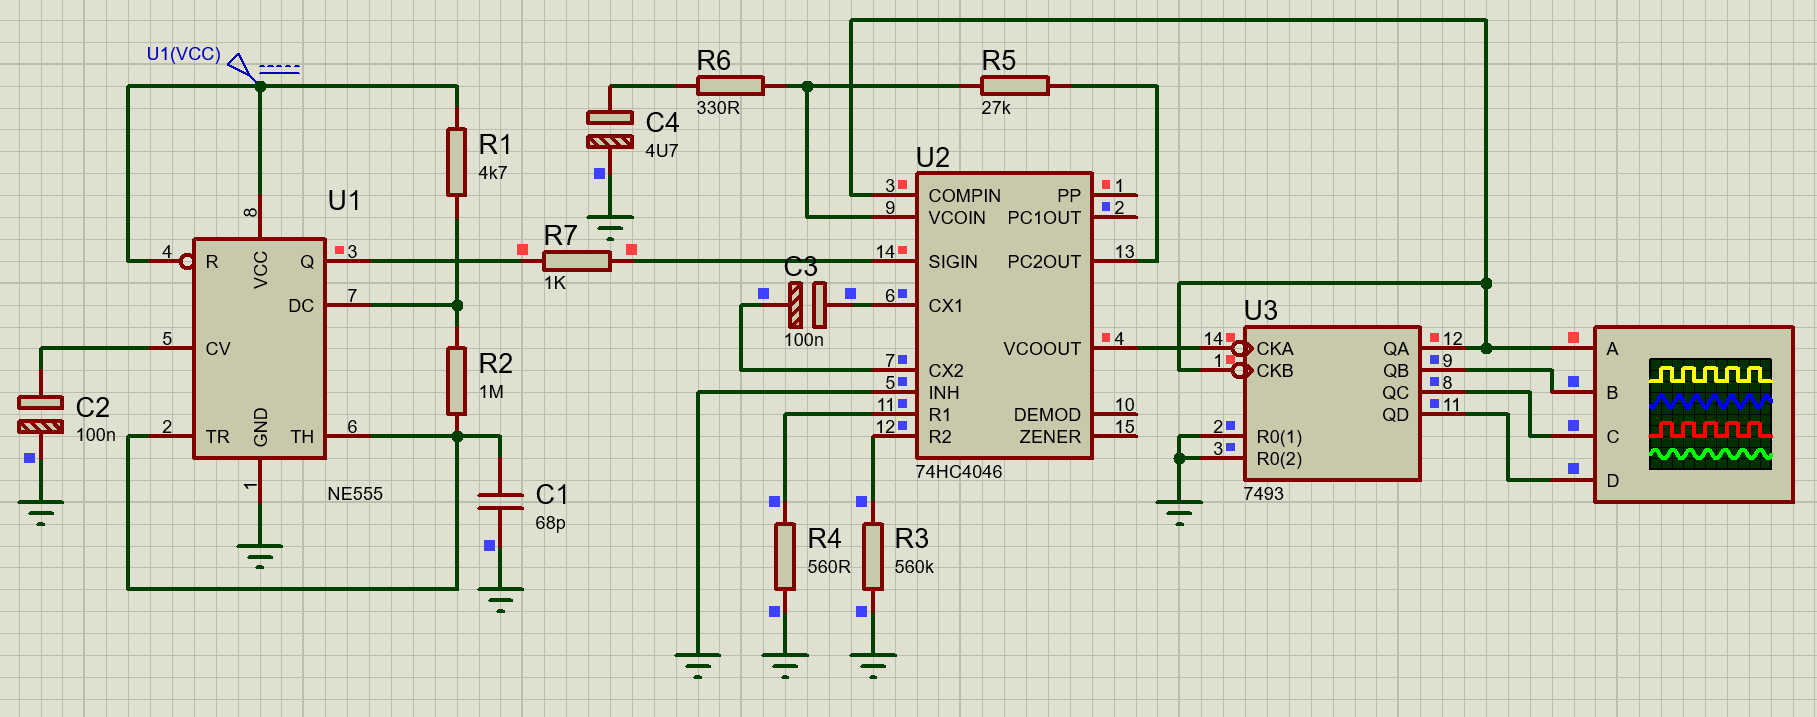
\includegraphics[width=.9\textwidth]{imgs/3.5. Esquemático.png}
        \caption{Simulación utilizando un 7493}
    \end{figure}
    {\it Nota: El resistor R7 fue colocado para evitar errores de convergencia en la simulación, no es necesario en una aplicación real.}
    \begin{figure}[H]
        \centering
        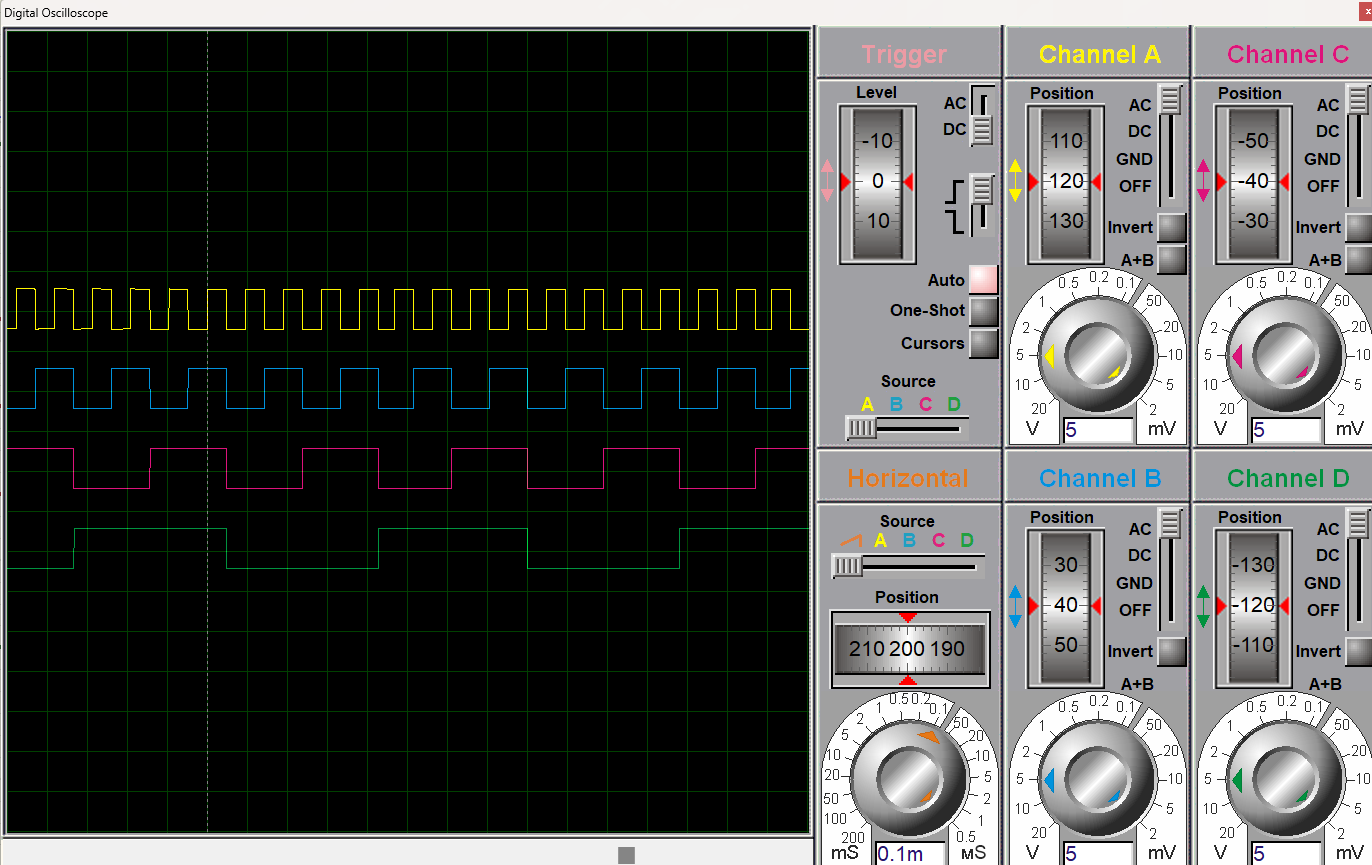
\includegraphics[width=.9\textwidth]{imgs/3.5. Osciloscopio.png}
        \caption{Osciloscopio simulado}
    \end{figure}
    Como se ve, el 7493 permite la división de la señal de entrada con los factores de x1, x, x4 y x8 las cuáles se pueden elegir para ser retroalimentadas al comparador de fase y conseguir el mismo factor pro de multiplicación para la salida del VCO. Si se desease otro valor operando los 4 bits de salida, se requeriría un circuito lógico de control adicional.
    \begin{figure}[H]
        \centering
        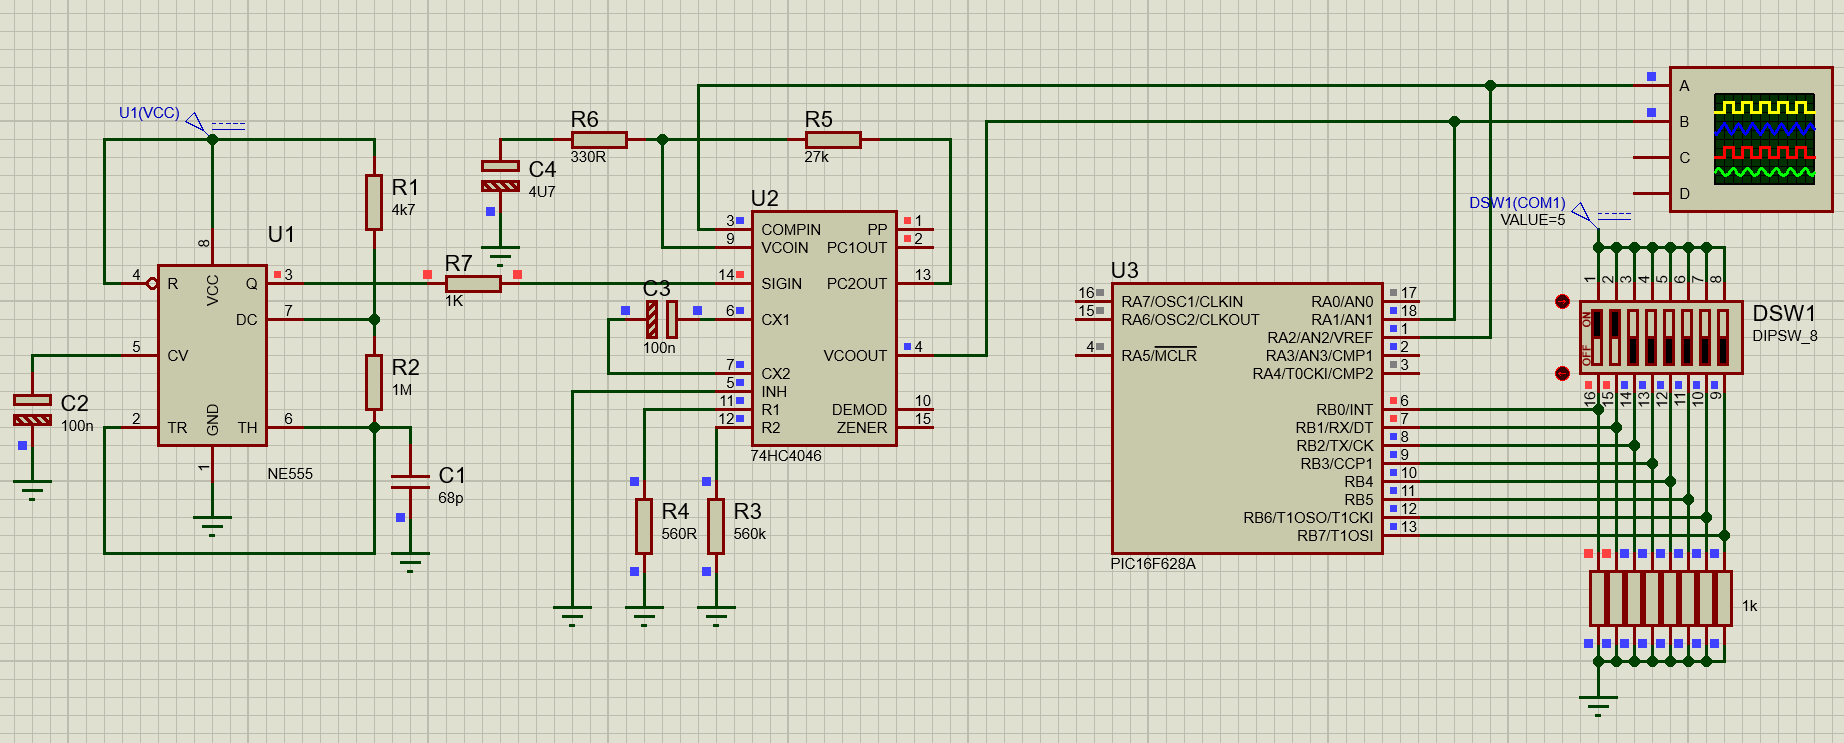
\includegraphics[width=.9\textwidth]{imgs/3.5. Simulación con PIC.png}
        \caption{Divisor de frecuencia usando un PIC16F628A16F628A}
    \end{figure}
    {\it Nota: El resistor R7 fue colocado para evitar errores de convergencia en la simulación, no es necesario en una aplicación real.}
\end{enumerate}
\section{MATERIAL Y EQUIPO}

\begin{itemize}
    \item 01 Fuente de Alimentación.
    \item 01 PLL LM565
    \item 01 contador 7490
    \item Resistencias según circuitos
    \item Condensadores según circuitos
    \item 01 Osciloscopio
    \item 01 cristal
    \item Generador de RF
    \item DIP switch
    \item Multímetro
\end{itemize}
\newpage
\section{PROCEDIMIENTO}
\begin{enumerate} [label={\alph*.}]
    \item Armar el circuito oscilador diseñado, comprobar su frecuencia y amplitud de salida.
    \begin{figure}[H]
        \centering
        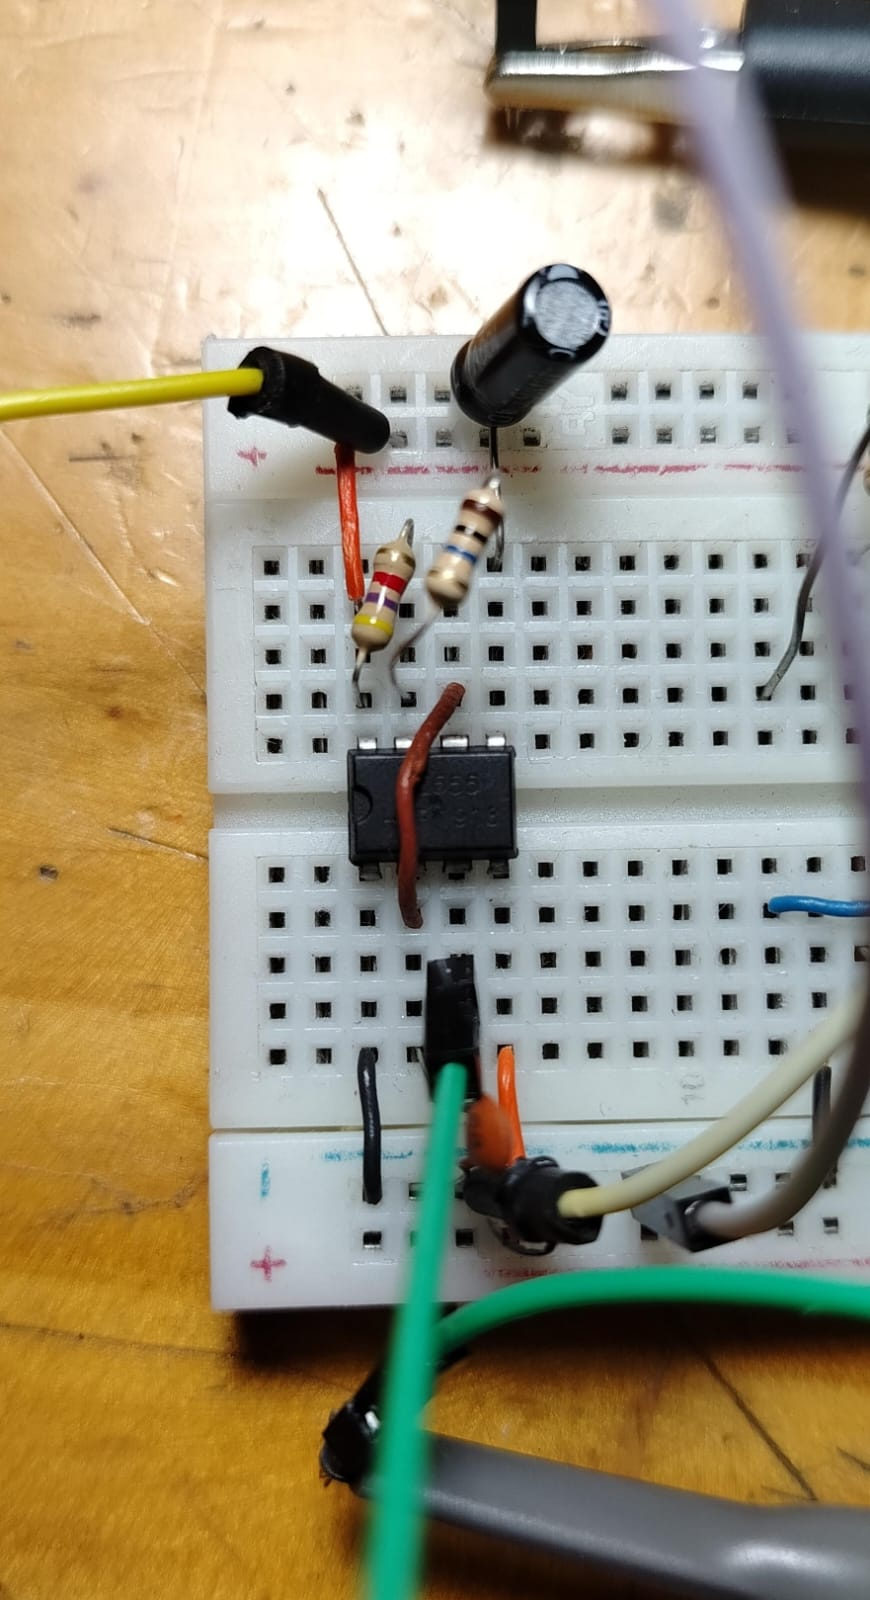
\includegraphics[width=.35\textwidth]{imgs/5.1. Circuito.jpg}
        \caption{Oscilador con NE555}
    \end{figure}
    \begin{figure}[H]
        \centering
        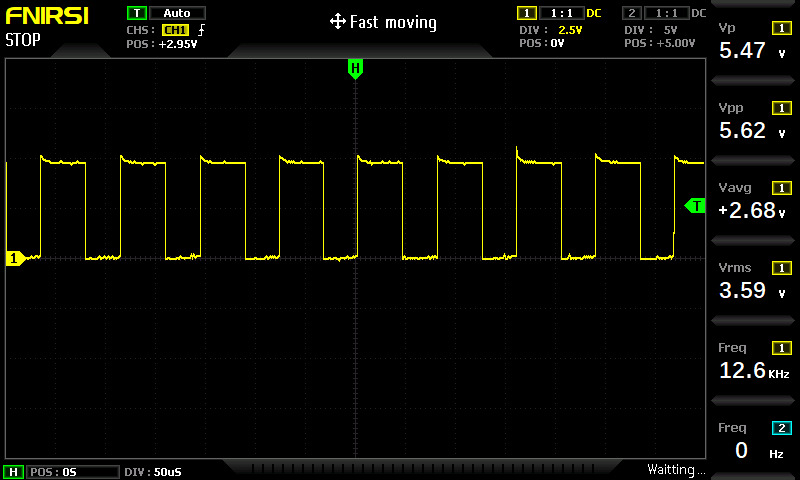
\includegraphics[width=.9\textwidth]{imgs/5.1. Osciloscopio del circuito.jpg}
        \caption{salida del oscilador}
    \end{figure}
    \item Armar el circuito de la Fig. 2, aplicar la señal de salida del oscilador, alimentar el circuito y observar la señal de salida en el osciloscopio.
    \begin{figure}[H]
        \centering
        \includegraphics[width=.9\textwidth]{imgs/5.2. CIrucito.jpg}
        \caption{Sintetizador con un PLL y un 7493}
    \end{figure}
    \begin{figure}[H]
        \centering
        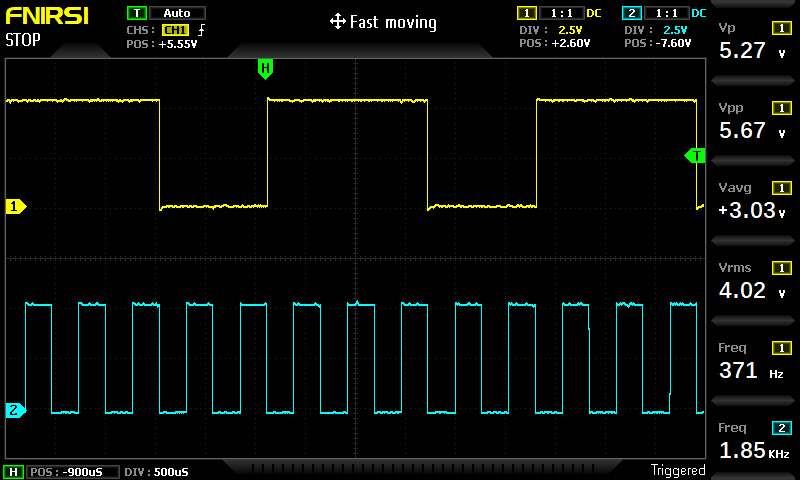
\includegraphics[width=.9\textwidth]{imgs/5.2. Salida del circuito.jpg}
        \caption{Comparación entre la entada del demodulador de fase y el VCO (división x4)}
    \end{figure}
    \newpage
    \begin{figure}[H]
        \centering
        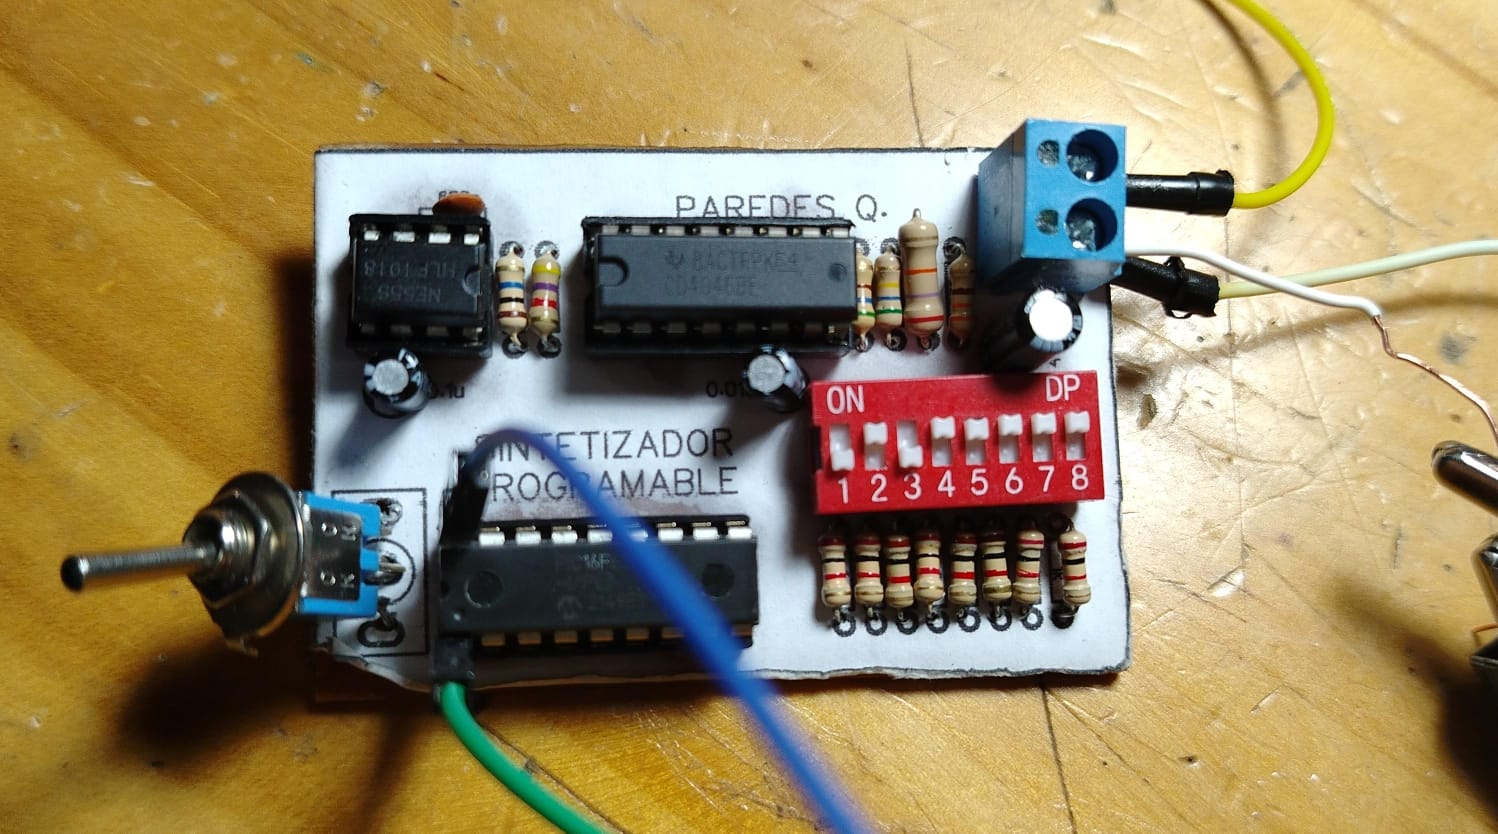
\includegraphics[width=.9\textwidth]{imgs/5.2. Cirucito con PIC.jpg}
        \caption{Sintetizador con un PLL y un PIC16F628A}
    \end{figure}
    \begin{figure}[H]
        \centering
        \includegraphics[width=.9\textwidth]{imgs/5.2. Salida PIC.jpg}
        \caption{Comparación entre la entada del demodulador de fase y el VCO (cambio cada 3 flancos)}
    \end{figure}
    \newpage
    \item Hacer un cambio de la amplitud de la señal de salida del oscilador, observar la salida y modificar hasta obtener la mejor señal de salida y anotar resultados de amplitud y frecuencia.
    \begin{figure}[H]
        \centering
        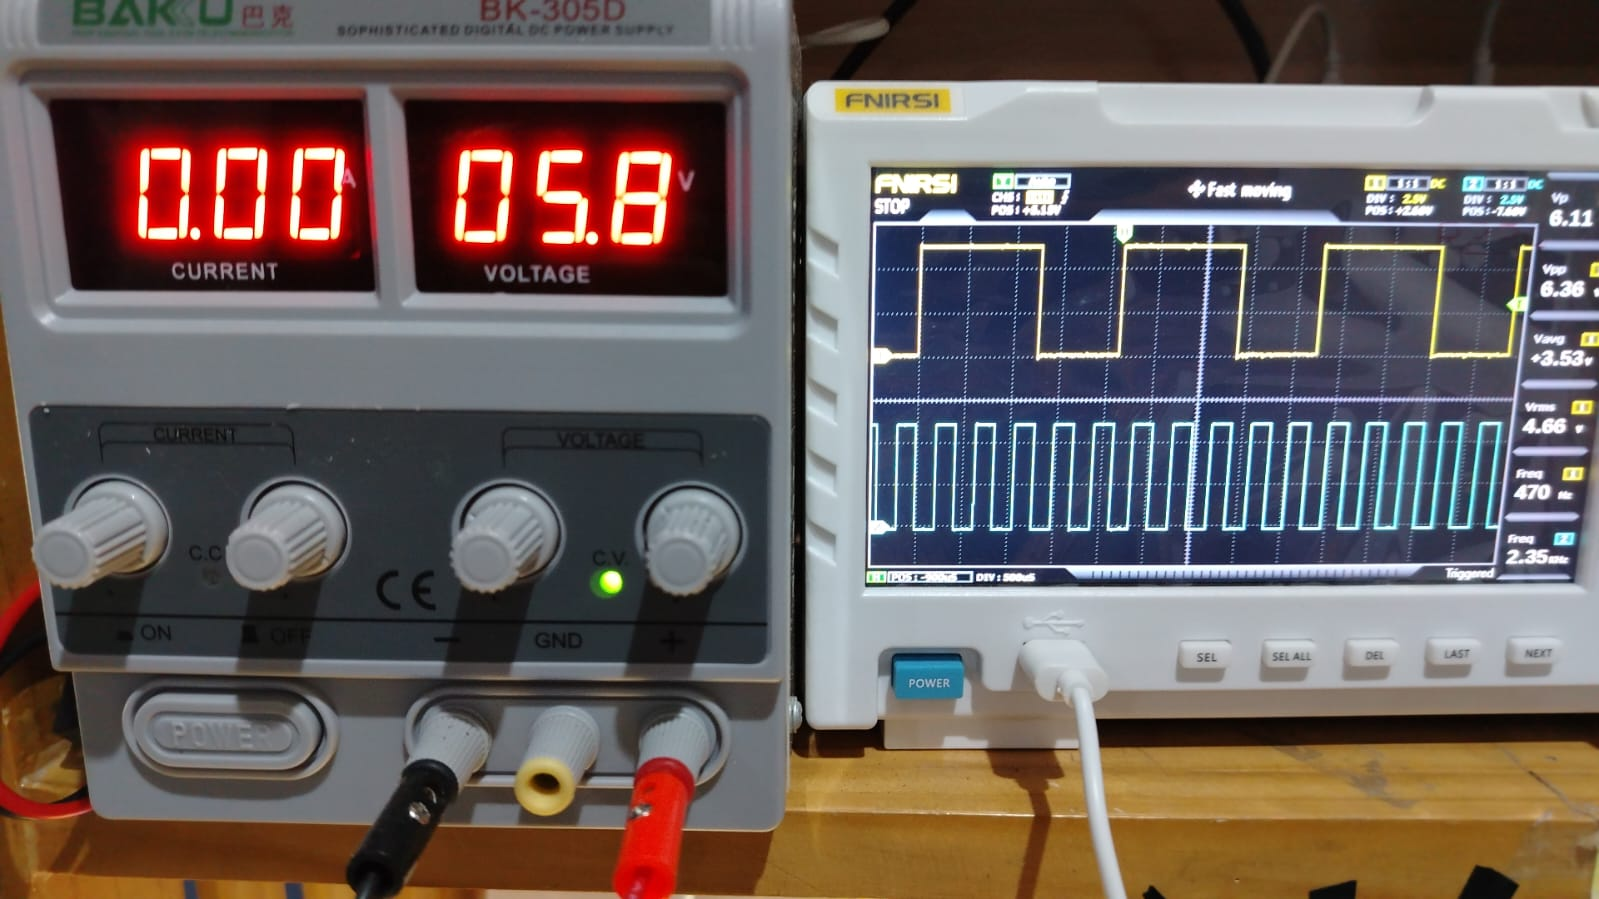
\includegraphics[width=.9\textwidth]{imgs/5.3. Nueva salida.jpg}
        \caption{Incremento de amplitud}
    \end{figure}
    Se incrementó la alimentación del sistema que dispone del 7493 (no se hizo esta variación en el sistema del PIC por cuidar el microcontrolador), lo condujo a un incremento de la amplitud de la salida del oscilador. Como se observa, todas las señales variaron en su amplitud pero no en frecuencia ni fase.
    \item Modificar el circuito contador para una división de menor valor.
    \begin{figure}[H]
        \centering
        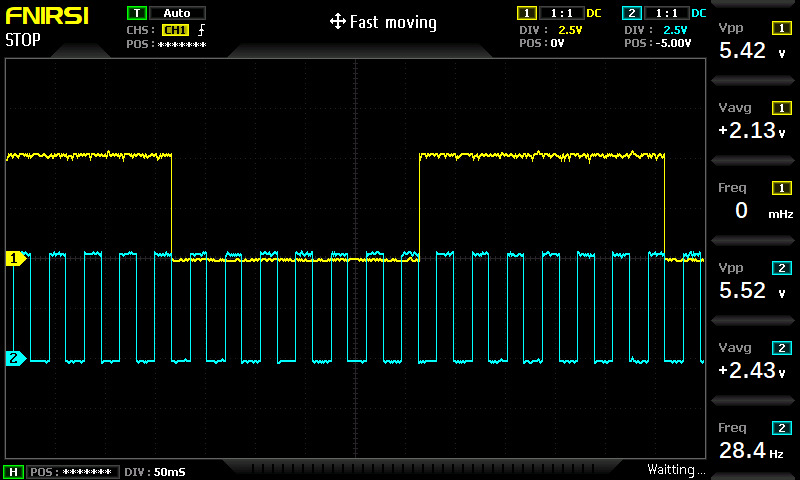
\includegraphics[width=.8\textwidth]{imgs/5.5. Menos frecuencia.jpg}
        \caption{División con PIC, cuenta 1 flanco para cambiar de estado}
    \end{figure}
    \item Modificar el circuito contador para una división de mayor valor
    \begin{figure}[H]
        \centering
        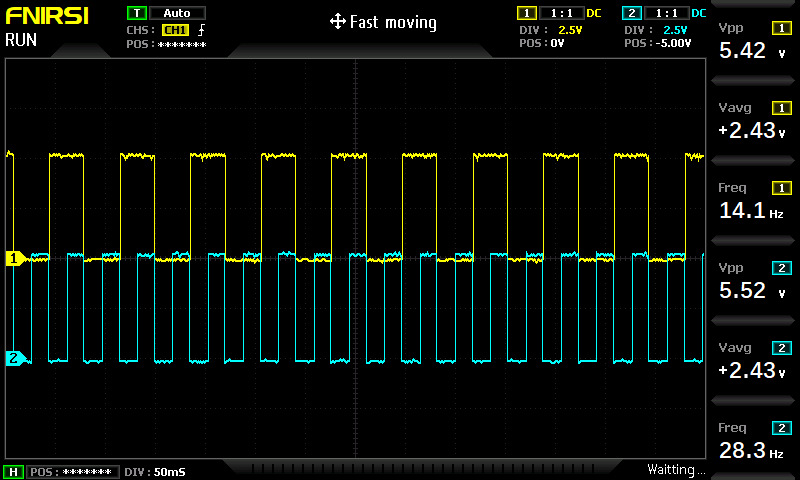
\includegraphics[width=.8\textwidth]{imgs/5.6. Más frecuencia.jpg}
        \caption{División con PIC, cuenta 7 flancos para cambiar de estado}
    \end{figure}
\end{enumerate}

\section{TAREAS COMPLEMENTARIAS}

Para analizar los parámetros de los sintetizadores de receptores de radio comercial FM, de TV comercial y de aparatos celulares móviles, es importante comprender las características y requisitos específicos de cada tipo de receptor.

\subsection{Receptores de Radio Comercial FM}

\begin{itemize}
    \item \textbf{Rango de Frecuencia:} 
    \begin{itemize}
        \item 88 a 108 MHz: Este es el rango de frecuencia estándar para la radio FM comercial.
    \end{itemize}
    \item \textbf{Estabilidad de Frecuencia:} 
    \begin{itemize}
        \item ±50 ppm: La estabilidad de frecuencia es crucial para mantener la sintonización precisa en el rango de FM.
    \end{itemize}
    \item \textbf{Ruido de Fase:} 
    \begin{itemize}
        \item Bajo ruido de fase: Es esencial para evitar la distorsión y mantener la calidad del audio. Típicamente, se espera que el ruido de fase esté por debajo de -100 dBc/Hz a 10 kHz de offset.
    \end{itemize}
    \item \textbf{Resolución de Frecuencia:} 
    \begin{itemize}
        \item 100 kHz o menor: Permite una sintonización precisa dentro del canal de FM.
    \end{itemize}
    \item \textbf{Tiempo de Bloqueo (Lock Time):} 
    \begin{itemize}
        \item Menos de 100 ms: El tiempo que tarda el PLL en estabilizarse en la frecuencia deseada.
    \end{itemize}
    \item \textbf{Desviación de Frecuencia:} 
    \begin{itemize}
        \item ±75 kHz: La desviación de frecuencia máxima permitida en la modulación de FM.
    \end{itemize}
\end{itemize}

\subsection{Receptores de TV Comercial}

\begin{itemize}
    \item \textbf{Rango de Frecuencia:} 
    \begin{itemize}
        \item 54 a 806 MHz: Dependiendo de la región y el estándar (NTSC, PAL, SECAM), el rango puede variar.
    \end{itemize}
    \item \textbf{Estabilidad de Frecuencia:} 
    \begin{itemize}
        \item ±10 ppm o mejor: La estabilidad es crucial para evitar la deriva de frecuencia y mantener la sintonización precisa.
    \end{itemize}
    \item \textbf{Ruido de Fase:} 
    \begin{itemize}
        \item Bajo ruido de fase: Similar a los receptores de FM, el ruido de fase bajo es importante para evitar la interferencia y mantener la calidad de la señal de video.
    \end{itemize}
    \item \textbf{Resolución de Frecuencia:} 
    \begin{itemize}
        \item 1 MHz o menor: Para sintonizar los diferentes canales de TV.
    \end{itemize}
    \item \textbf{Tiempo de Bloqueo (Lock Time):} 
    \begin{itemize}
        \item Menos de 50 ms: El tiempo de bloqueo rápido es necesario para cambiar de canal rápidamente.
    \end{itemize}
    \item \textbf{Sensibilidad del Receptor:} 
    \begin{itemize}
        \item Menos de -85 dBm: La sensibilidad adecuada asegura una recepción clara incluso en condiciones de señal débil.
    \end{itemize}
\end{itemize}

\subsection{Aparatos Celulares Móviles}

\begin{itemize}
    \item \textbf{Rango de Frecuencia:} 
    \begin{itemize}
        \item 700 MHz a 2600 MHz: Dependiendo de la banda de operación (2G, 3G, 4G, 5G), los rangos de frecuencia pueden variar.
    \end{itemize}
    \item \textbf{Estabilidad de Frecuencia:} 
    \begin{itemize}
        \item ±0.1 ppm: Los teléfonos móviles requieren una estabilidad de frecuencia extremadamente alta debido a la necesidad de mantener la sincronización con la red celular.
    \end{itemize}
    \item \textbf{Ruido de Fase:} 
    \begin{itemize}
        \item Muy bajo ruido de fase: Es crítico para mantener la calidad de la señal y evitar la interferencia con otros canales y dispositivos. Valores típicos están por debajo de -120 dBc/Hz a 10 kHz de offset.
    \end{itemize}
    \item \textbf{Resolución de Frecuencia:} 
    \begin{itemize}
        \item 1 kHz o mejor: Permite una sintonización precisa y ajuste fino de la frecuencia portadora.
    \end{itemize}
    \item \textbf{Tiempo de Bloqueo (Lock Time):} 
    \begin{itemize}
        \item Menos de 1 ms: Los dispositivos móviles deben poder cambiar frecuencias rápidamente para manejar el traspaso de llamadas y datos entre celdas.
    \end{itemize}
    \item \textbf{Ancho de Banda del Canal:} 
    \begin{itemize}
        \item 1.4 MHz a 20 MHz: Dependiendo del estándar (LTE, 5G), el ancho de banda del canal puede variar significativamente.
    \end{itemize}
    \item \textbf{Sensibilidad del Receptor:} 
    \begin{itemize}
        \item -100 dBm o mejor: La alta sensibilidad es necesaria para recibir señales débiles y mejorar la calidad de la llamada y la transmisión de datos.
    \end{itemize}
\end{itemize}

\subsection{Consideraciones Comunes}

\begin{itemize}
    \item \textbf{Linealidad y Desviación de la Fase:} Para todos estos sistemas, es crucial que los sintetizadores mantengan una linealidad alta y una desviación de fase mínima para asegurar la calidad de la señal.
    \item \textbf{Consumo de Energía:} Especialmente para dispositivos móviles, el consumo de energía es una consideración importante para prolongar la vida útil de la batería.
    \item \textbf{Interferencias y Aislamiento:} La capacidad de aislar y minimizar las interferencias es esencial para todos los dispositivos que operan en un entorno electromagnético denso.
\end{itemize}

\section{CUESTIONARIO FINAL}

\begin{enumerate} [label={\arabic*)}]
    \item Presentar los resultados del procedimiento y comparar con los simulados.\\
    Se obtuvieron los resultados esperados del informe previo en la sección de procedimiento.
    \item Fundamentar la multiplicación de frecuencia utilizando contadores y cuáles son sus límites.\\
    La división de frecuencia con contadores funciona al tener que esperar una cantidad exponencial de 2 (para contadores binarios) de pulsos en la entrada para tener un cambio de estado en la salida. El número de contadores que se coloquen en cadena determinará la cantidad de pulsos a esperar. Si se desea algún valor que no sea de la escala exponencial de 2, se requiere un circuito lógico adicional que controle el reinicio del conteo.
    \item ¿Qué componentes podrían mejorar la magnitud de respuesta de división y/o multiplicación de frecuencia?\\
    El PLL CD4046 usando en la práctica funciona utilizando un voltaje TTL, lo que evita su optimización en la magnitud de respuesta, al ser esta ya muy estable para los voltajes TTL  lógicos (5V activo y 0 inactivo). Además, esta estabilidad es compartida por el comparador de fase, lo que permite que filtros sencillos, como el empleado en la práctica de un cero y un polo, sean suficientes. Incluso, el fabricante recomiendo el uso de filtros de orden 1, pues los de orden superior no tienen un gran impacto en el funcionamiento de los circuitos con el PLL CD4046. Sin embargo, una mejora que se puso en práctica fue el uso de un microcontrolador para la división de frecuencias programable de amplio rango. Con un mejor microcontrolador y un circuito más complejo (como uno con doble oscilador y doble divisor de frecuencias, programable y no programable) se podría tener una resolución mínima, un muy grande ancho de banda (rango de frecuencia disponibles) y una respuesta veloz y estable.
    \item Indicar en que aplicaciones prácticas de estos circuitos.\\
    Los circuitos sintetizadores con PLL tienen una amplia gama de aplicaciones prácticas en diversas áreas de la electrónica.
    \begin{enumerate}
        \item Telecomunicaciones:
        \begin{itemize}
            \item Generación de Frecuencias: En sistemas de telecomunicaciones, los PLL se utilizan para generar señales de referencia de alta frecuencia y para sintetizar frecuencias de portadora precisas.
            \item Modulación y Demodulación: Los PLL se emplean en moduladores y demoduladores de frecuencia, fase y amplitud para asegurar la coherencia de fase entre las señales transmitidas y recibidas.
        \end{itemize}
        \item Radiofrecuencia (RF):
        \begin{itemize}
            \item Sintonización de Radio: En receptores de radio, los PLL se usan para sintonizar frecuencias específicas de estaciones de radio con gran precisión.
            \item Osciladores Locales: Los PLL se utilizan en osciladores locales de receptores y transmisores de RF para estabilizar y ajustar frecuencias.
        \end{itemize}
        \item Relojes de Sistemas Digitales:
        \begin{itemize}
            \item Generación de Relojes: En sistemas digitales, los PLL generan señales de reloj de alta frecuencia a partir de una referencia de baja frecuencia, asegurando que todos los componentes del sistema funcionen en sincronía.
            \item Distribución de Relojes: Los PLL también se utilizan para distribuir señales de reloj a diferentes partes de un sistema digital con mínimas variaciones de fase (jitter).
        \end{itemize}
        \item Sistemas de Audio y Video:
        \begin{itemize}
            \item Sincronización de Video: En sistemas de video, los PLL se usan para sincronizar la señal de video con la fuente de referencia, asegurando la estabilidad de la imagen.
            \item Sistemas de Audio Digital: En equipos de audio digital, los PLL ayudan a mantener la sincronización entre diferentes componentes, evitando distorsiones y pérdidas de calidad.
        \end{itemize}
        \item Redes de Comunicaciones:
        \begin{itemize}
            \item En redes de comunicación, los PLL se emplean para mantener la sincronización entre nodos de red, esencial para la transmisión de datos sin errores.
            \item Multiplexación por División de Frecuencia (FDM): Los PLL se utilizan para sintetizar las diferentes frecuencias portadoras en sistemas FDM, permitiendo la transmisión de múltiples señales a través de un solo canal.
        \end{itemize}
    \end{enumerate}:
\end{enumerate}
\section{CONCLUSIONES Y OBSERVACIONES}

{\it Indicar las Conclusiones y observaciones}

\begin{itemize}
    \item Se diseñaron y construyeron 2 circuitos sintetizadores a base de lógica TTL y un microcontrolador.
    \item Se pudo comparar las bondades que ofrece cada sistema, en términos de costo de implementación y capacidades.
    \item Se logró diseñar un oscilador en base a un NE555.
    \item Se comprendió más sobre las aplicaciones de los circuitos sintetizadores basados en PLL.
    \item Se comprendió el diseño e implementación de divisores de frecuencia.
\end{itemize}

\section{BIBLIOGRAFIA}
\begin{thebibliography}{00}
\bibitem{NE555}
Analog Devices. “Calculadora Para Temporizador 555  | DigiKey Electronics.” Digikey.com.mx, 2023, \url{www.digikey.com.mx/es/resources/conversion-calculators/conversion-calculator-555-timer}.

\bibitem{PLL}
Miyara, Federico, and Universidad Nacional De Rosario. PLL LAZOS de FIJACIÓN de FASE 2000 Rosario TEL 0341 4808543 Argentina FAX 0341 4802654 ELECTRÓNICA III. \url{https://www.fceia.unr.edu.ar/enica3/pll.pdf}

\end{thebibliography}
\section{ANEXOS} 
Código del PIC16F628A

\begin{minted}[linenos, bgcolor=lightgray, fontsize=\small, breaklines]{c}
// CONFIG
#pragma config FOSC = INTOSCIO  // Oscillator Selection bits (INTOSC oscillator: I/O function on RA6/OSC2/CLKOUT pin, I/O function on RA7/OSC1/CLKIN)
#pragma config WDTE = OFF       // Watchdog Timer Enable bit (WDT disabled)
#pragma config PWRTE = OFF      // Power-up Timer Enable bit (PWRT disabled)
#pragma config MCLRE = OFF      // RA5/MCLR/VPP Pin Function Select bit (RA5/MCLR/VPP pin function is digital input, MCLR internally tied to VDD)
#pragma config BOREN = ON       // Brown-out Detect Enable bit (BOD enabled)
#pragma config LVP = OFF        // Low-Voltage Programming Enable bit (RB4/PGM pin has digital I/O function, HV on MCLR must be used for programming)
#pragma config CPD = OFF        // Data EE Memory Code Protection bit (Data memory code protection off)
#pragma config CP = OFF         // Flash Program Memory Code Protection bit (Code protection off)

#include <xc.h>

#define _XTAL_FREQ 4000000  // Set the internal oscillator frequency to 4MHz

void main() {
    TRISA = 0b11110011;
    TRISB = 0xFF;
    CMCON = 0b00000111;
    __delay_ms(10);
    
    unsigned int counter = 0;
    unsigned char target = 0;

    while(1) {
        while (PORTAbits.RA1 == 1) {}
        
        counter++;
        target = PORTB;
        if(counter >= target) {
            counter = 0;
            PORTAbits.RA2 = !PORTAbits.RA2;
        }
        
        while (PORTAbits.RA1 == 0) {}
    }
}
\end{minted}

DISEÑO DEL PCB
\begin{figure}[H]
    \centering
    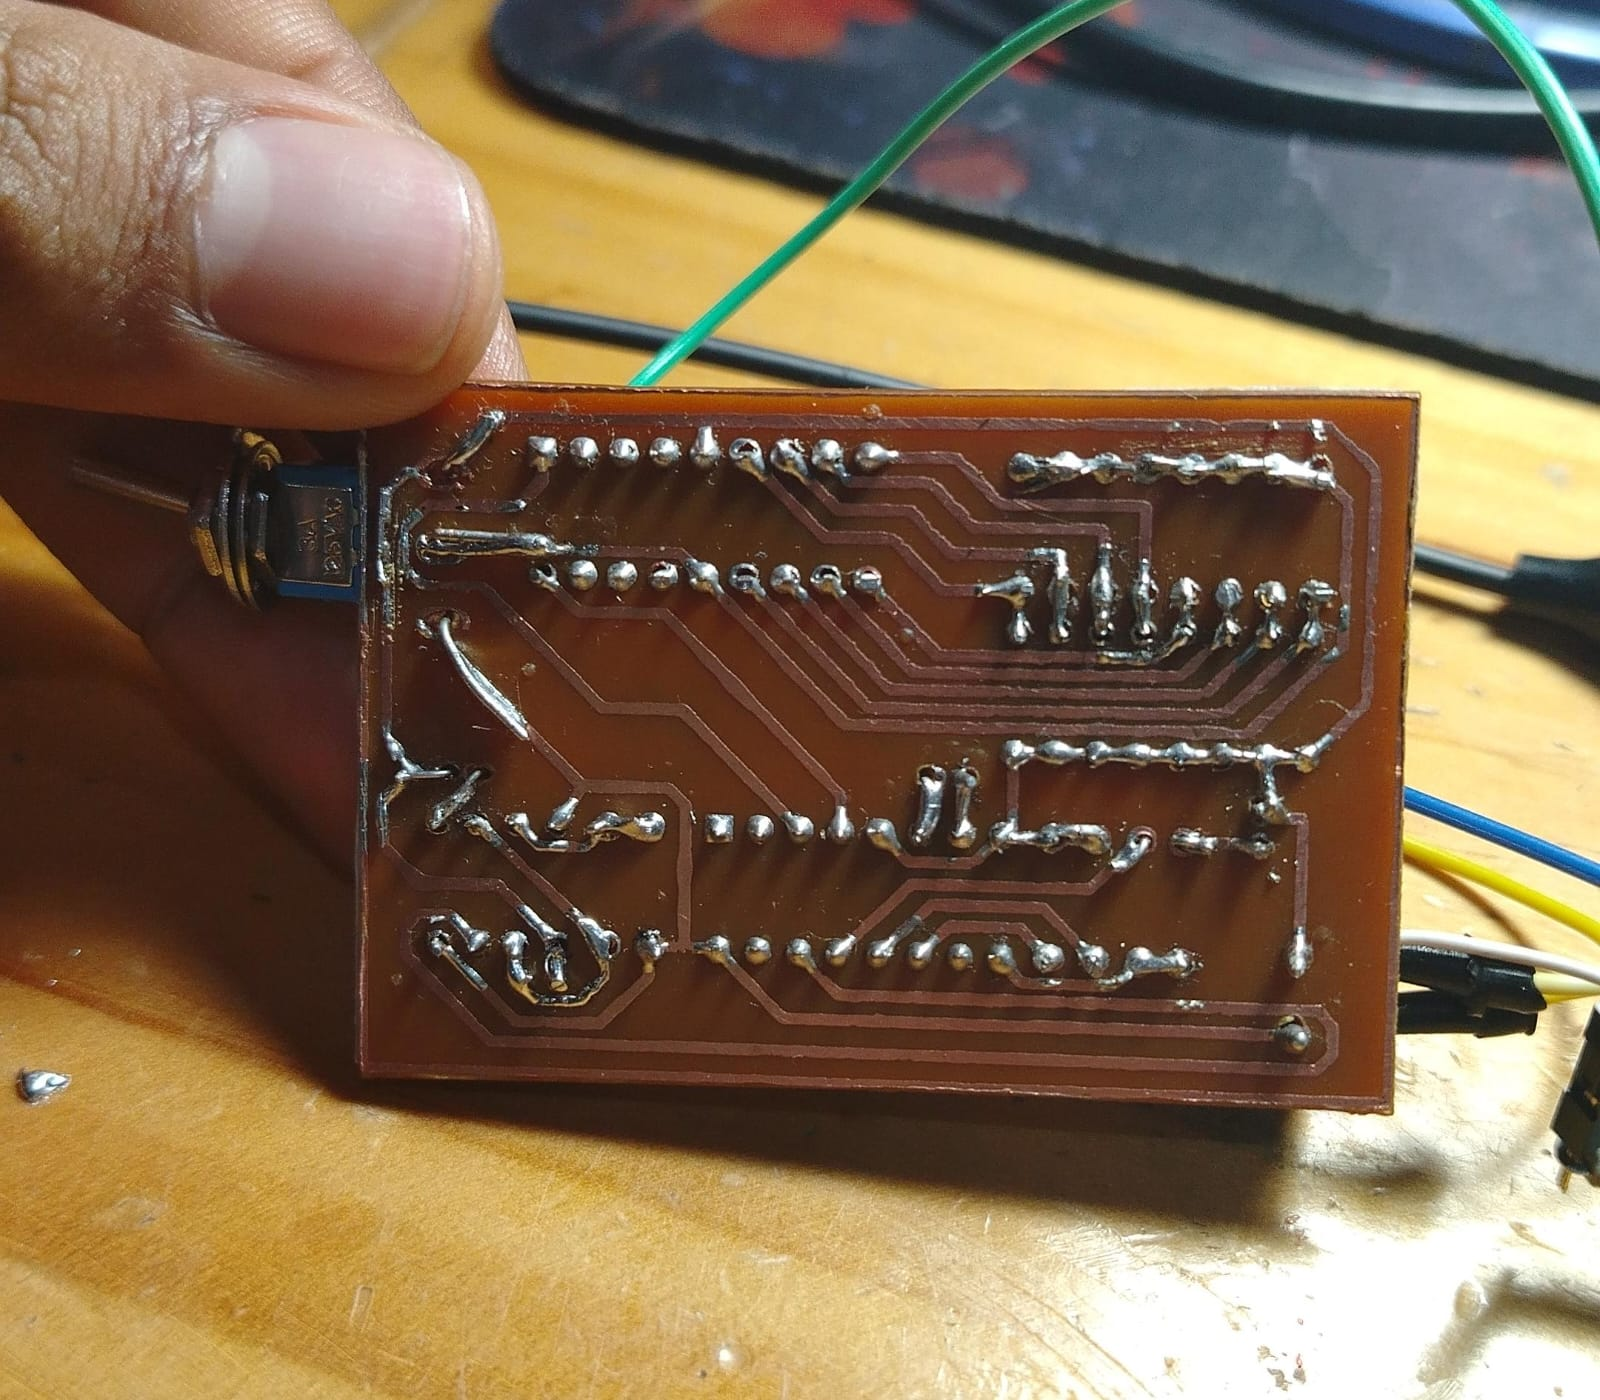
\includegraphics[width=.7\textwidth]{imgs/ANEXO PCB.jpg}
    \caption{PCB IMPRESO}
\end{figure}
\begin{figure}[H]
    \centering
    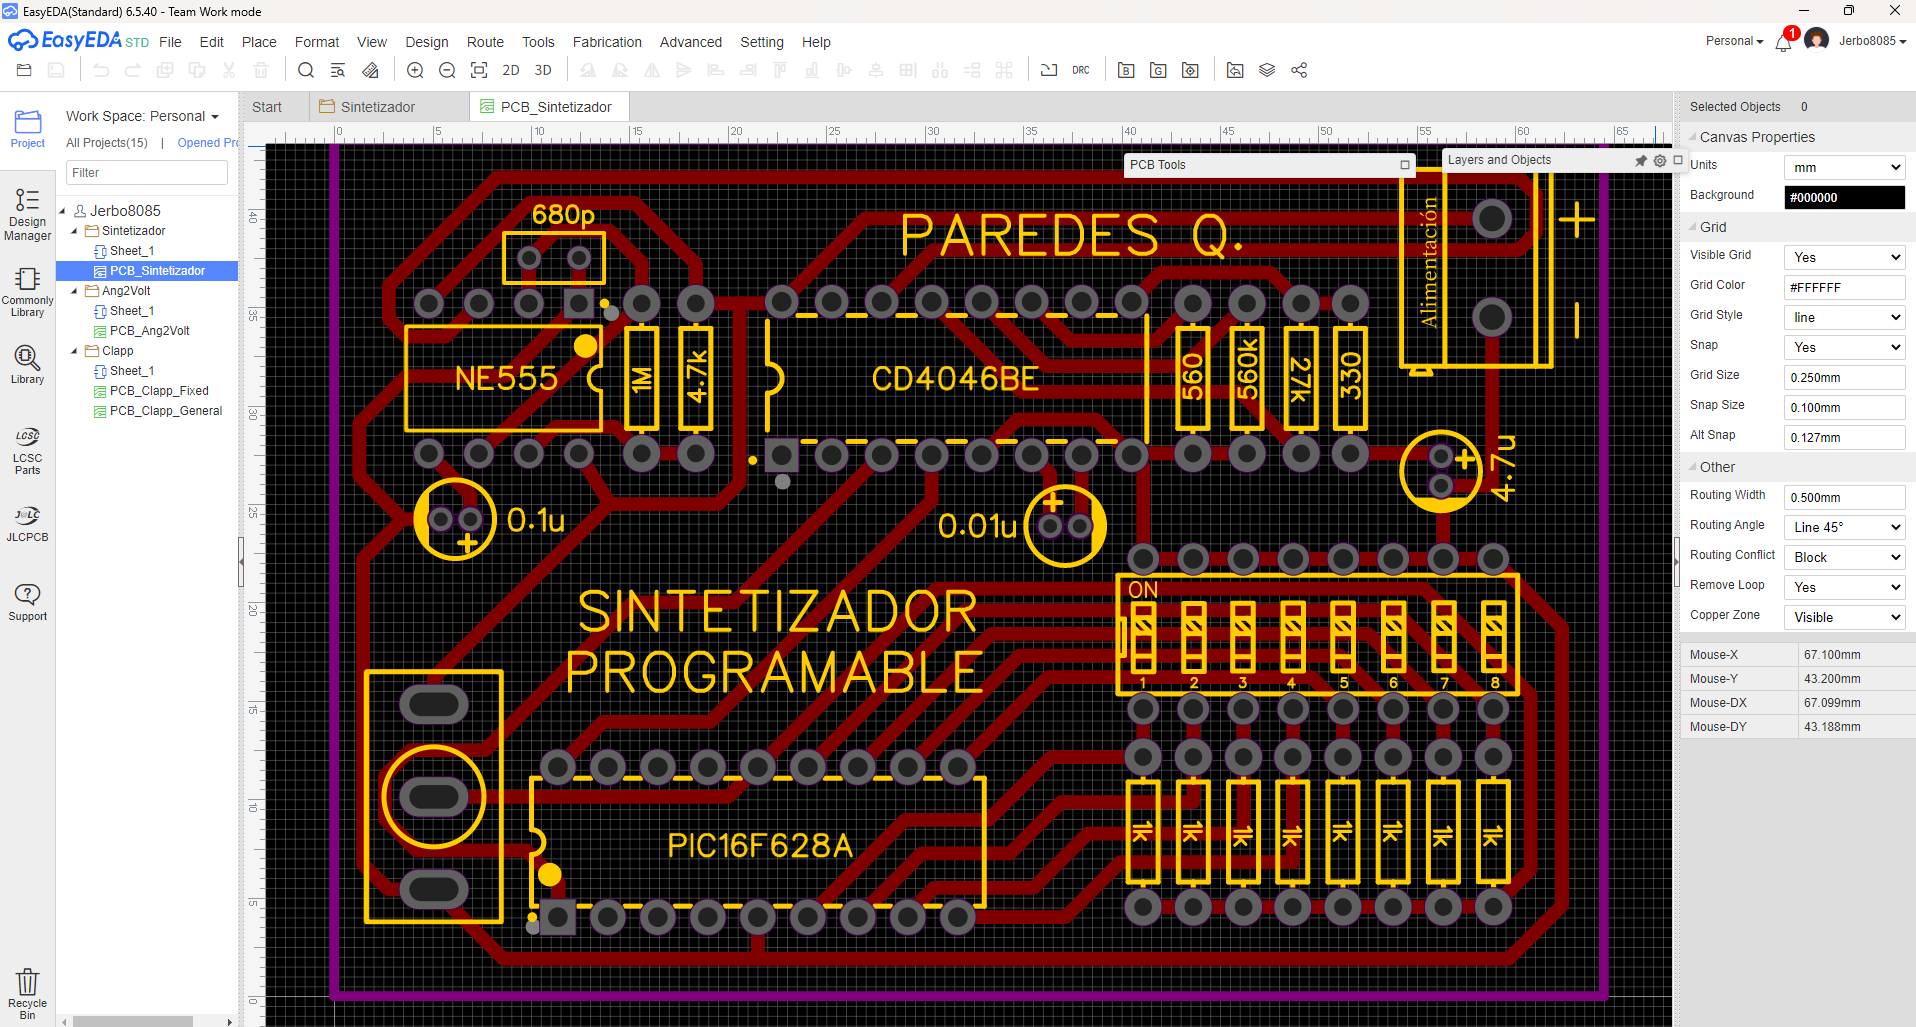
\includegraphics[width=.7\textwidth]{imgs/ANEXO PCB 2.png}
    \caption{PCB DISEÑO}
\end{figure}

\end{document}
